%%  export TEXINPUTS=.:/home/mjw/src/manuals/common:

\documentclass[11pt,a4paper,openany,oneside]{book}

\usepackage{hyperref} 
\usepackage{listings}
\usepackage{graphicx}
\usepackage{parskip}
\usepackage{enumitem}
\usepackage{latexsym}

\newcommand{\ci}[1]{\hspace*{1cm} {\small\texttt{#1}}}
\newcommand{\cc}[1]{{\texttt{#1}}}
% Set bullet style
\renewcommand{\labelitemi}{$\Box$} 

\newenvironment{description*}%
  {\setlength{\parskip}{0pt}%
	 \begin{description}%
		\setlength{\topsep}{-12pt}%
		\setlength{\itemindent}{-12pt}%
    \setlength{\itemsep}{0pt}%
		\setlength{\itemsep}{0pt}}%
  {\end{description}}

\newenvironment{enumerate*}%
  {\begin{enumerate}%
		\setlength{\topsep}{-12pt}%
		\setlength{\itemindent}{-12pt}%
    \setlength{\itemsep}{0pt}%
		\setlength{\parindent}{0pt}}%
  {\end{enumerate}}
  
\begin{document}

\begin{titlepage}

\begin{center}
{\Huge OpenTTP manual}
\end{center}

\vspace*{4cm}
\begin{center}
Version 1.0
\end{center}

\begin{center}
Copyright 2016 OpenTTP
\end{center}

\end{titlepage}

\tableofcontents
\listoffigures
\listoftables

\lstset{
	xleftmargin=24pt,
	basewidth=0.5em,
	basicstyle=\ttfamily,
	escapechar=\%
}

%% ****************************************************************************************
\chapter{Introduction}
%% ****************************************************************************************

\section{What is OpenTTP?}

\section{GPS common-view}

\section{The OpenTTP reference platform}

\section{Supported hardware}

	\subsection{GNSS receivers}
	
	\begin{table}
	\begin{tabular}{lll}
	Manufacturer & models & notes \\ \hline
	Javad & GRIL receivers & obsolete \\
	NVS   & NV08 & \\
	Trimble & Resolution T & obsolete\\
	ublox & Neo8MT & \\
	\end{tabular}
	\caption{Supported GPS/GNSS receivers.}
	\end{table}
	
	Note: OpenTTP uses a custom file format for logging GPS receiver data. It does not read native receiver binary-format files.
	
	Guidance on testing a receiver for suitability for time-transfer, and writing software to process
	the receiver's data, is given in the OpenTTP Developer's Guide.
	
	\subsection{Counter/timers}
	
	\begin{table}
	\begin{tabular}{lll}
	Manufacturer & models & notes \\ \hline
	Agilent & 5313x &  needs IOTech GPIB to RS232 converter\\
	OpenTTP &  & \\
	SRS & PRS10 & uses input 1 pps time-tagging function\\
	\end{tabular}
	\caption{Supported counter/timers.}
	\end{table}
	
%% ****************************************************************************************
\chapter{Getting started}
%% ****************************************************************************************

\section{Software installation requirements}

In addition to a basic Linux development environment, you will need the development packages for:
\begin{description*}
	\item[\cc{boost}]   
	\item[\cc{libgsl}] GNU scientific library
\end{description*}

Depending on your Linux installation, you may also need
\begin{description*}
	\item[\cc{Time::HiRes}] Perl library
\end{description*}

\section{Building and installing the software}

Two scripts are provided for installing the software.
\begin{lstlisting}
software/system/installsys.pl
software/gpscv/install.pl
\end{lstlisting}

\cc{installsys.pl} must be run first, because it installs libraries which are needed by the GPSCV software.

Run-time options can be viewed by running the script with the '-h' option. In particular, \cc{installsys.pl}
has options to list the available installation targets and to install particular targets.

\section{A minimal software setup}

Some users may only be interested in the core software that OpenTTP provides so that they can use
it with their own hardware. This section describes the minimum setup required for operation.

The OpenTTP software distribution is comprised of various C/C++ applications and Perl scripts.
As a minimum, you will need:
\begin{description*}
	\item \cc{TFLibrary.pm} Perl module for commonly used tasks, such as reading configuration files
	\item \cc{libconfigurator} C library for parsing configuration files
	\item \cc{lockport} utility to create a UUCP lock file
	\item \cc{mktimetx} creates time-transfer files
	\item one of the OpenTTP-provided scripts to log your receiver
	\item one of the OpenTTP-provided scripts to log your counter/timer
\end{description*}

You must use one of the OpenTTP receiver logging scripts because \cc{mktimetx} expects a custom file-format. In particular, the
receiver's native binary formats are not readable by \cc{mktimetx}. Similarly, OpenTTP uses a custom file
format for the counter-timer measurement files, although in this case, conversion from another format
will probably be straight-forward. Most likely, users will have to provide their own software for
logging their counter/timer, given the large number of possible devices here, and the limited
support within OpenTTP.

You may find the following useful:
\begin{description*}
	\item[] \cc{kickstart.pl} for automatic start of logging processes
	\item[] \cc{runmktimetx.pl} for automated processing, and reprocessing
	\item[] \cc{ziplogs.pl} for log file compression
\end{description*}	

Sample configuration files can be found in \cc{software/gpscv/common/etc}.
The user running the logging and processing needs the following directories (or equivalents - most paths
can be configured via the general configuration file, \ref{sgpscvconf}):
\cc{bin}, \cc{cggtts},\cc{etc},\cc{logs},\cc{raw},\cc{rinex},\cc{tmp}.

%% ****************************************************************************************
\chapter{System hardware}
%% ****************************************************************************************


\begin{figure}
\centerline{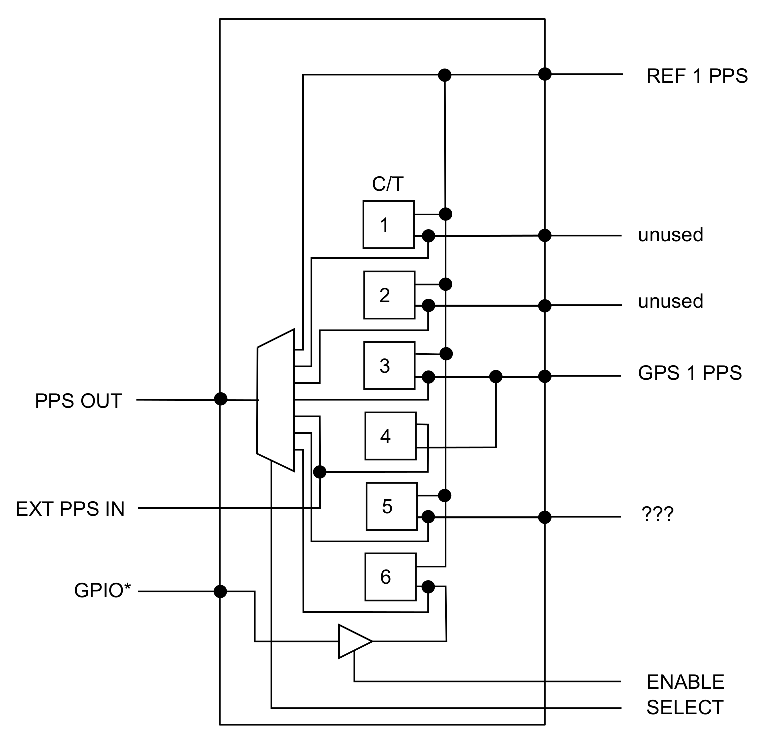
\includegraphics{figures/ottpcounter.eps}}
\end{figure}

\begin{table}
\begin{center}
\begin{tabular}[lll]
1 & channel 1 pps & unused\\
2 & channel 2 pps & GNSS receiver\\
3 & channel 3 pps & unused\\
4 & channel 4 pps & \\
5 & channel 5 pps & \\
6 & channel 6 pps & GPIO\\
7 & GPIO enabled\\
8 & Digital Clock Manager PLL is locked\\
\end{tabular}
\end{center}
\end{table}


%% ****************************************************************************************
\chapter{GPSCV software}
%% ****************************************************************************************

\section{Configuration file format \label{sConfigFileFormat}}

Configuration files use a common format and are plain text files, designed to be easily edited via a command-line
editor because in many applications, only shell access to the system will be available.

The file is divided into sections, with section names delimited by square brackets [ ]. Entries in each section
are of the form:
\begin{lstlisting}
key = value
\end{lstlisting}
For example,
\begin{lstlisting}
[Receiver]
manufacturer = Trimble
model = Resolution T
\end{lstlisting}
defines a section `Receiver' and the receiver's manufacturer and model. 
The notation \cc{Section::Key} is used to describe keys. For example,
\cc{Receiver::model} and \cc{Receiver::manufacturer} describe the two keys above.

Keys and section names are not case-sensitive. Comments begin with a '\#'.

Some keys define a list of sections. For example, the comma-separated list of values for 'outputs' 
\begin{lstlisting}
[CGGTTS]
outputs = C1-code,P1-code,P2-code
\end{lstlisting}
defines three sections: \cc{C1-code}, \cc{P1-code}, and \cc{P2-code}.

\section{gpscv.conf - the core configuration file \label{sgpscvconf} }

A single configuration file, \cc{gpscv.conf}, provides configuration information to most of the
OpenTTP software. 
\cc{gpscv.conf} is used by \cc{mktimetx}, receiver logging scripts, TIC logging scripts,receiver utilities and so on.

It uses the format described in \ref{sConfigFileFormat}.

\begin{table}[h]
\begin{tabular}{l|p{10cm}}
Section & Key \\ \hline
\hyperlink{h:antenna}{Antenna} & antenna number, antenna type, 
				delta H, delta N, delta E, frame,
				marker name, marker number,
				X, Y, Z\\ \hline
\hyperlink{h:cggtts}{CGGTTS} & BIPM cal id, comments, create, 
         ephemeris, ephemeris file, ephemeris path,
         internal delay, lab id, maximum DSG, minimum elevation,
         minimum track length, naming convention, outputs, reference,
         receiver id, revision date, version,
         code, constellation, path
         \\ \hline
\hyperlink{h:delays}{Delays}  & antenna cable, reference cable 
         \\ \hline
\hyperlink{h:counter}{Counter} & file extension, GPIB address, header generator, lock file,
         logger, logger options, okxem channel, port
				\\ \hline
\hyperlink{h:misc}{Misc}    & gzip
				\\ \hline
\hyperlink{h:paths}{Paths} & CGGTTS, counter data, processing log, receiver data, RINEX, tmp
				\\ \hline
\hyperlink{h:receiver}{Receiver} & configuration, elevation mask, logger, logger options, 
				 manufacturer, model, observations, 
         port, pps offset, synchronization, pps synchronization delay,
         status file, timeout, version
				\\ \hline
\hyperlink{h:reference}{Reference} & file extension, logging interval, log path, log status, oscillator, power flag, status file
        \\ \hline
\hyperlink{h:rinex}{RINEX}  & agency, create, observer, version
				\\ \hline
\end{tabular}
\caption{Summary of \cc{gpscv.conf} entries}
\end{table}

\subsection{[Antenna] section}

\hypertarget{h:antenna}{}
{\bfseries antenna number}\\
This appears as ANTNUM in the RINEX header.\\
\textit{Example:}
\begin{lstlisting}
antenna number=A567456
\end{lstlisting}

{\bfseries antenna type}\\
This appears as ANTTYPE in the RINEX header.\\
\textit{Example:}
\begin{lstlisting}
antenna type=Ashtec
\end{lstlisting}

{\bfseries delta H}\\
This appears as DELTA H in the RINEX header.\\
\textit{Example:}
\begin{lstlisting}
delta H=0.0
\end{lstlisting}

{\bfseries delta E}\\
This appears as DELTA E in the RINEX header.\\
\textit{Example:}
\begin{lstlisting}
delta E=0.0
\end{lstlisting}

{\bfseries delta N}\\
This appears as DELTA N in the RINEX header.\\
\textit{Example:}
\begin{lstlisting}
delta N=0.0
\end{lstlisting}

{\bfseries frame}\\
This appears as FRAME in the CGGTTS header.\\
\textit{Example:}
\begin{lstlisting}
frame= ITRF2010
\end{lstlisting}

{\bfseries marker name}\\
This appears as MARKER NAME in the RINEX header.\\
\textit{Example:}
\begin{lstlisting}
marker name=
\end{lstlisting}

{\bfseries marker number}\\
This appears as MARKER NUMBER in the RINEX header.\\
\textit{Example:}
\begin{lstlisting}
marker number=
\end{lstlisting}

{\bfseries X}\\
This appears as X in the CGGTTS header and APPROX POSITION XYZ in the RINEXheader.\\
\textit{Example:}
\begin{lstlisting}
X=+4567890.123
\end{lstlisting}

{\bfseries Y}\\
This appears as Y in the CGGTTS header and APPROX POSITION XYZ in the RINEXheader.\\
\textit{Example:}
\begin{lstlisting}
Y=+2345678.90
\end{lstlisting}

{\bfseries Z}\\
This appears as Z in the CGGTTS header and APPROX POSITION XYZ in the RINEXheader.\\
\textit{Example:}
\begin{lstlisting}
Z=-1234567.890 
\end{lstlisting}


\subsection{[CGGTTS] section }

\hypertarget{h:cggtts}{Entries} in this section control the format and content of CGGTTS files and filtering applied to CGGTTS tracks.

{\bfseries BIPM cal id}\\
This defines CAL\_ID for the internal delay, as used in v2E CGGTTS headers.\\
\textit{Example:}
\begin{lstlisting}
BIPM cal id=none
\end{lstlisting}

{\bfseries comments}\\
This defines COMMENTS in the CGGTTS header.\\
\textit{Example:}
\begin{lstlisting}
comments=none
\end{lstlisting}

{\bfseries create}\\
This defines whether or not CGGTTS files will be generated.\\
\textit{Example:}
\begin{lstlisting}
create=yes
\end{lstlisting}

{\bfseries ephemeris}\\
This defines whether to use the receiver-provided ephemeris or a user-provided ephemeris (via a RINEX navigation file).
If a user-provided ephemeris is specified then \cc{ephemeris path} and \cc{ephemeris file} 
must also be specified.\\
\textit{Example:}
\begin{lstlisting}
ephemeris=receiver
\end{lstlisting}

{\bfseries ephemeris file}\\
This specifies a pattern for user-provided RINEX navigation files.
Currently, only patterns of the form \cc{XXXXddd0.yyn} are recognized.\\
\textit{Example:}
\begin{lstlisting}
ephemeris file=SYDNddd0.yyn
\end{lstlisting}

{\bfseries ephemeris path}\\
This specifies the path to user-provided RINEX navigation files.\\
\textit{Example:}
\begin{lstlisting}
ephemeris path=igsproducts
\end{lstlisting}

{\bfseries internal delay}\\
This defines INT DLY in the CGGTTS header. The units are ns.\\
\textit{Example:}
\begin{lstlisting}
INT DLY=0.0
\end{lstlisting}

{\bfseries lab id}\\
This defines the two-character lab code used for creating BIPM-style file names, as per the V2E specification.\\
\textit{Example:}
\begin{lstlisting}
lab id=AU
\end{lstlisting}

{\bfseries maximum DSG}\\
CGGTTS tracks with DSG lower than this will be filtered out. 
The units are ns.\\
\textit{Example:}
\begin{lstlisting}
maximum DSG = 10.0
\end{lstlisting}

{\bfseries minimum elevation}\\
CGGTTS tracks lower than this will be filtered out. 
The units are degrees.\\
\textit{Example:}
\begin{lstlisting}
minimum elevation = 10
\end{lstlisting}

{\bfseries minimum track length}\\
CGGTTS tracks shorter than this will be filtered out. Tracks meeting the criterion are not necessarily contiguous.
The units are seconds.\\
\textit{Example:}
\begin{lstlisting}
minimum track length = 390
\end{lstlisting}

{\bfseries naming convention}\\
Defines the CGGTTS file naming convention. Valid options are `plain' (MJD.cctf) and `BIPM'.
The \cc{lab id} and \cc{receiver id} should be defined in conjunction with BIPM-style filenames.\\
\textit{Example:}
\begin{lstlisting}
naming convention = BIPM
\end{lstlisting}

{\bfseries outputs}\\
This defines a list of sections which in turn define the desired CGGTTS outputs.\\
\textit{Example:}
\begin{lstlisting}
outputs=CGGTTS-GPS-C1,CGGTTS-GPS-P1,CGGTTS-GPS-P2
\end{lstlisting}

{\bfseries reference}\\
This defines REF in the CGGTTS header.\\
\textit{Example:}
\begin{lstlisting}
reference=UTC(XXX)
\end{lstlisting}

{\bfseries receiver id}\\
This defines the two-character receiver code used for creating BIPM-style file names, 
as per the V2E specification.\\
\textit{Example:}
\begin{lstlisting}
receiver is=01
\end{lstlisting}

{\bfseries revision date}\\
This defines REV DATE in the CGGTTS header. It must be in the format YYYY-MM-DD.\\
\textit{Example:}
\begin{lstlisting}
revision date = 2015-12-31
\end{lstlisting}

{\bfseries version}\\
This defines the version of CGGTTS output.Valid versions are v1 and v2E. 
The \cc{lab id} and \cc{receiver id} should be defined in conjunction with v2E ouput\\
\textit{Example:}
\begin{lstlisting}
version = v2E
\end{lstlisting}

\subsubsection{CGGTTS output sections}

Multiple CGGTTS outputs can be defined, allowing for different constellation and signal combinations.
An example of a CGGTTS output section is as follows:
\begin{lstlisting}
[CGGTTS-GPS-C1]
constellation=GPS
code=C1
path=cggtts
BIPM cal id = none
internal delay = 11.0
\end{lstlisting}

The new entries for a CGGTTS output section are:\\
{\bfseries code}\\
This defines the GNSS signal code. Valid values are C1,P1 and P2.\\
\textit{Example:}
\begin{lstlisting}
code=C1
\end{lstlisting}

{\bfseries constellation}\\
This defines the GNSS constellation. Only GPS is supported currently.\\
\textit{Example:}
\begin{lstlisting}
constellation=GPS
\end{lstlisting}

{\bfseries path}\\
This defines the directory in which output files are placed.\\
\textit{Example:}
\begin{lstlisting}
path=cggtts
\end{lstlisting}

\subsection{[Counter] section}

\hypertarget{h:counter}{}

{\bfseries file extension}\\
This defines the extension used for time interval measurement files.
The default is `tic'.\\
\textit{Example:}
\begin{lstlisting}
file extension=tic
\end{lstlisting}

{\bfseries GPIB address}\\
For GPIB devices, the GPIB address must be defined.
\textit{Example:}
\begin{lstlisting}
GPIB address=3
\end{lstlisting}

{\bfseries header generator}\\
A header for the log file can be optionally added to the log file, using the output
of a user provided script. Output should be to \cc{stdout}.
Each line will have a ``\#'' automatically prepended to it.\\
\textit{Example:}
\begin{lstlisting}
header generator=bin/myticheader.pl
\end{lstlisting}

{\bfseries lock file}\\
This defines the device lock file, used to prevent multiple instances of the logger
from being started.\\
\textit{Example:}
\begin{lstlisting}
lockfile = okxem.gpscv.lock
\end{lstlisting}

{\bfseries logger}\\
This defines the counter logging script.\\
\textit{Example:}
\begin{lstlisting}
logger=okxemlog.pl
\end{lstlisting}

{\bfseries logger options}\\
This defines options passed to the counter logging script.\\
\textit{Example:}
\begin{lstlisting}
logger options=
\end{lstlisting}

{\bfseries okxem channel}\\
The OpenTTP counter is multi-channel so the channel to use (1-6) must be specified.\\
\textit{Example:}
\begin{lstlisting}
okxem channel=3
\end{lstlisting}

{\bfseries port}\\
This defines the port used to communicate the counter. It's value depends on the type of counter. 
For the XEM6001, it's a Unix socket. For serial devices, it's a device name like
\cc{/dev/ttyUSB0}.\\
\textit{Example:}
\begin{lstlisting}
# this is the port used by okcounterd
port = 21577 
\end{lstlisting}

\subsection{[Misc section}

\hypertarget{h:misc}{}

{\bfseries gzip}\\
Defines the compression/decompression program used in conjunction with counter and receiver log files.\\
\textit{Example:}
\begin{lstlisting}
gzip=/bin/gzip 
\end{lstlisting}

\subsection{[Delays] section}

\hypertarget{h:delays}{}

{\bfseries antenna cable}\\
This is ANT DLY as used in the CGGTTS header. Units are ns.\\
\textit{Example:}
\begin{lstlisting}
antenna cable=0.0
\end{lstlisting}

{\bfseries reference cable}\\
This is REF DLY as used in the CGGTTS header. Units are ns.\\
\textit{Example:}
\begin{lstlisting}
reference cable=0.0
\end{lstlisting}

\subsection{[Paths] section}

\hypertarget{h:paths}{Paths} are relative to the user's home directory, unless prefaced with a `/', in which case
they are interpreted as absolute paths.

{\bfseries CGGTTS}\\
Defines the default directory used for CGGTTS files.\\
\textit{Example:}
\begin{lstlisting}
CGGTTS=cggtts
\end{lstlisting}

{\bfseries counter data}\\
Defines the directory used for TIC data files.\\
\textit{Example:}
\begin{lstlisting}
counter data=
\end{lstlisting}

{\bfseries processing log}\\
Defines the directory where the \cc{mktimetx} processing log is written.\\
\textit{Example:}
\begin{lstlisting}
processing log=logs
\end{lstlisting}

{\bfseries receiver data}\\
Defines the directory used for GNSS receiver raw data files.\\
\textit{Example:}
\begin{lstlisting}
receiver data=raw
\end{lstlisting}

{\bfseries RINEX}\\
Defines the directory used for RINEX files.\\
\textit{Example:}
\begin{lstlisting}
RINEX=rinex
\end{lstlisting}

{\bfseries tmp}\\
Defines the directory used for intermediate and debugging files.\\
\textit{Example:}
\begin{lstlisting}
tmp=tmp
\end{lstlisting}


\subsection{[Receiver] section \label{sgcreceiver}}

\hypertarget{h:receiver}{}

{\bfseries configuration}\\
\\
\textit{Example:}
\begin{lstlisting}
configuration = etc/rx.conf
\end{lstlisting}

{\bfseries elevation mask}\\
This sets an elevation mask for tracking os satellites - below this elevation, satellites
are ignored. The units are degrees. This may not be implemented for all receivers.\\
\textit{Example:}
\begin{lstlisting}
elevation mask = 0
\end{lstlisting}

{\bfseries logger}\\
This is the script used to configure and log messages from the GNSS receiver.\\
\textit{Example:}
\begin{lstlisting}
logger = jnslog.pl
\end{lstlisting}

{\bfseries logger options}\\
These are options passed to the receiver logging script.\\
\textit{Example:}
\begin{lstlisting}
logger options =
\end{lstlisting}

{\bfseries manufacturer}\\
This defines the manufacturer of the receiver. Together with the model and version, 
this sets how data from the receiver is processed. For a list of supported receivers
see XX.\\
\textit{Example:}
\begin{lstlisting}
manufacturer = Javad
\end{lstlisting}

{\bfseries model}\\
This is the receiver model.For a list of supported receivers
see XX.\\
\textit{Example:}
\begin{lstlisting}
model = HE_GGD
\end{lstlisting}

{\bfseries observations}\\
This is a list of GNSS systems tracked by the receiver. Only GPS is supported
at present. Although the receiver model defines the possible observations,
it may be configured to track only one GNSS system, so this entry specifies which
one is being tracked.\\
\textit{Example:}
\begin{lstlisting}
observations = GPS
\end{lstlisting}

{\bfseries port}\\
This is the serial port used for communication with the receiver.\\
\textit{Example:}
\begin{lstlisting}
port = /dev/ttyS0
\end{lstlisting}

{\bfseries pps offset}\\
This is an offset programmed into the GNSS receiver. Its purpose is to ensure that the counter
triggers correctly, particularly HP5313x counters, which will only trigger every two seconds if the 
start trigger slips slightly behind the stop trigger. It is only useful though if the reference 
(which by convention is Start) has comparable long-term stability with GPS eg a GPSDO or Cs beam standard.
The units are ns.\\
\textit{Example:}
\begin{lstlisting}
pps offset = 3500
\end{lstlisting}

{\bfseries pps synchronization}\\
This is a Javad-specific option. The logging script will force a synchronization of the receiver's
internal time scale with the input 1 pps.\\
\textit{Example:}
\begin{lstlisting}
pps synchronization = no
\end{lstlisting}

{\bfseries pps synchronization delay}\\
This is a Javad-specific option. Synchronization of the receiver's
internal time scale with the input 1 pps is delayed for this time after reset of the receiver.
The units are seconds.\\
\textit{Example:}
\begin{lstlisting}
pps synchronization delay = 300
\end{lstlisting}

{\bfseries status file}\\
\\
\textit{Example:}
\begin{lstlisting}
status file =
\end{lstlisting}

{\bfseries timeout}\\
The logging script will time out and exit if no messages are received for this period.\\
\textit{Example:}
\begin{lstlisting}
timeout = 60
\end{lstlisting}

{\bfseries version}\\
This can be used to identify the firmware version in use, for example.\\
\textit{Example:}
\begin{lstlisting}
version = 2.6.1
\end{lstlisting}

\subsection{[Reference] section}

\hypertarget{h:reference}{}

{\bfseries file extension}\\
This defines the extension used for Reference status logs.\\
\textit{Example:}
\begin{lstlisting}
file extension= .rb
\end{lstlisting}

{\bfseries logging interval}\\
This defines the interval between status file updates. The units are seconds.\\
\textit{Example:}
\begin{lstlisting}
logging interval=60
\end{lstlisting}

{\bfseries log path}\\
This defines where status logs are written to.\\
\textit{Example:}
\begin{lstlisting}
log path=raw
\end{lstlisting}

{\bfseries log status}\\
This enables status logging of the Reference.\\
\textit{Example:}
\begin{lstlisting}
log status=yes
\end{lstlisting}

{\bfseries oscillator}\\
This identifies the installed oscillator, so that device-specific handling can be implemented.\\
\textit{Example:}
\begin{lstlisting}
oscillator=PRs10
\end{lstlisting}

{\bfseries power flag}\\
This defines the file used to flag that the Reference has lost power, and needs rephasing.
Currently, this only has meaning for the PRS10. It is used ntpd to disable the refclock
corresponding to the PRs10's 1 pps.\\
\textit{Example:}
\begin{lstlisting}
power flag=logs/prs10.pwr
\end{lstlisting}

{\bfseries status file}\\
In the case of the PRS10, this consists of the six status bytes and sixteen ADC values.\\
\textit{Example:}
\begin{lstlisting}
status file=logs/prs10.status
\end{lstlisting}


\subsection{[RINEX] section}

\hypertarget{h:rinex}{Entries} in this section control the format and content of RINEX files.

{\bfseries agency}\\
This specifies the value of the AGENCY field which appears in RINEX observation file headers.\\
\textit{Example:}
\begin{lstlisting}
agency=MY AGENCY
\end{lstlisting}

{\bfseries create}\\
This defines whether or not RINEX files will be generated.\\
\textit{Example:}
\begin{lstlisting}
create = yes
\end{lstlisting}

{\bfseries observer}\\
This specifies the value of the OBSERVER field which appears in RINEX observation file headers.
If the observer is specified as `user' then the environment variable USER is used.\\
\textit{Example:}
\begin{lstlisting}
observer=user
\end{lstlisting}

{\bfseries version}\\
This  specifies the version of the RINEX output. Valid versions are 2 and 3.\\
\textit{Example:}
\begin{lstlisting}
version=2
\end{lstlisting}





General notes

NVS

Note that this receiver uses UTC as the reference timescale to report time stamps.

This receiver reports a measurement time for observation a few hundred ms prior to the upcoming
second.

Trimble

 

Internals

One aspect to keep straight is that three timescales are used in the software:
PC time
UTC
GPS time

PC time is used to match TIC and GNSS observations. The time stamps recorded in measurement files do
not have a fractional seconds part. The latency of the various signals (eg GPS messages 
for a second are always output after the beginning of the second) and their logging by the host PC 
means that this is no ambiguity during normal operation.

UTC time is used for CGGTTS generation.

GPS time is used for various calculations and for RINEX observations.

\subsection{Application.cpp}

Matched measurements are stored in a vector whose index corresponds to UTC time-of-day.

\subsection{CGGTTS.cpp}


\section{Adding support for a new receiver}

\subsection{Conventions}

A counter/timer measurement must be started by REF and stopped by GPS.
There is an option in gpscv.conf to reverse the sign of this.

The sawtooth correction is ADDED to the counter/timer measurement.

\subsection{Configuring the receiver}

It may be necessary to turn off tracking of non-GPS GNSS systems.

It may be desirable to configure the receiver's refernce time scale 
\subsection{Clocks and pseudoranges}

When developing for a new receiver, interpreting the usually terse documentation can require
guesswork. The main problem is to make sure that you can establish the relationship between the raw 
pseudoranges and the output 1 pps. The receiver measurements will likely be reported with respect to the 
receiver clock, which will necessarily have an offset with respect to the refernec timescale.


It can be very helpful to have another, already-supported receiver on the same antenna. The pseudo ranges reported 
by this receiver can be used to identify any mysterious offsets in the pseudoranges 

\subsection{Sawtooth correction}

For CGGTTS output, the sawtooth correction may not have much effect at the 780s averaging time implicit in a CGGTTS track.

\subsection{Diagnostics}

Extra diagnostic files can be produced via command line options.
The option \cc{--timing-diagnostics} produces a text file \cc{timing.dat}. This text file has four columns:
	\begin{description*}
	\item[1] timestamp, in seconds since beginning of UTC day
	\item[2] TIC measurement, in seconds
	\item[3] 1 pps sawtooth correction, in seconds, to be added to the TIC measurement
	\item[4] receiver time offset, in seconds
	\end{description*}

The option \cc{--sv-diagnostics} produces a test file \cc{SVn.dat} for each GNSS satellite. This text file has
XXX columns
	\begin{description}
	\item[1] interpolated pseudo range
	\item[2] raw pseudo range
	\end{description}
	
\subsection{Debugging and validation}

It can be useful to look at how well the receiver recovers GPS time - this is easily done by
using the option --disable-tic. The sawtooth-corrected TIC measurement is then set to zero.

REFSYS values noisy at the hundreds of ns level may indicate an off by one error in assigned time stamps.




\cc{runmktimetx.pl} provides a convenient way to process multiple days of data and to run any missed processing.

	
\subsection{usage}
\cc{runmktimetx.pl} is normally run as a \cc{cron} job.

To run on the command line, use
\begin{lstlisting}
runmktimetx.pl [OPTION] \textellipsis [Start MJD  [Stop MJD]]
\end{lstlisting}
If an MJD or MJD range is not specified, the previous day is processed.

The options are
\begin{description*}
	\item[-d]	run in debugging mode
	\item[-h]	print help and exit
	\item[-x] run missed processing
	\item[-v]	print version information and exit
\end{description*}

\subsection{configuration file}
\cc{runmktimetx.pl} uses \cc{gpscv.conf}.

\subsection{log file}
\cc{runmktimetx.pl} doesn't produce a log file.

\section{Counter/timer logging scripts}

\subsection{hp5313xlog.pl}

There is a file \cc{hp5313x.cmds} which lists the SCPI commands used to configure the counter.
For example:
\begin{lstlisting}
:FUNC 'TINT 1,2'                # time interval
:SENS:EVEN1:LEVEL:ABS 1.0       # trigger level 1 volt
:SENS:EVEN2:LEVEL:ABS 1.0       #
:SENS:EVEN1:SLOP POS            # trigger on positive slope
:SENS:EVEN2:SLOP POS
:INP1:ATT 1                     # input attenuation x1
:INP2:ATT 1
:INP1:COUP DC                   # coupling DC
:INP2:COUP DC
:INP1:IMP 50                    # impedance 50 ohms
:INP2:IMP 50
\end{lstlisting}

\subsection{okxemlog.pl}

The OpenTTP reference platform includes a multi-channel TIC

It has the following specific configuration file entries:
It also uses:

\section{Receiver logging scripts}

\subsection{jnslog.pl}

There is a file \cc{receiver.conf} which lists the commands used to configure the receiver.

\subsection{nvslog.pl}

The NVS receiver is entirely configured using the script.

\subsection{restlog.pl}

The Resolution T receiver is entirely configured using the script.

\subsection{ubloxlog.pl}

The ublox receiver is entirely configured using the script.

\section{Receiver utilities}

\subsection{Trimble Resolution T}

\subsection{NVS NV08}

\subsection{ublox}

\subsection{Javad}


%% ****************************************************************************************
\chapter{System software}
%% ****************************************************************************************

\section{kickstart.pl}

\section{mjd}

\cc{mjd} provides conversion between a calendar date and MJD and shows the current MJD.

\subsection{usage}

\begin{lstlisting}[mathescape=true]
mjd [option]
\end{lstlisting}
The command line options are:
\begin{description*}
\item[-d \textless DD MM YYYY\textgreater] convert date to MJD
\item[-h] print help and exit
\item[-m \textless MJD\textgreater] convert MJD to date
\item[-t] print today's MJD and exit
\item[-v] print version information and exit
\end{description*}



\section{okcounterd \label{sokcounterd}}

\hypertarget{h:okcounterd}{}

\cc{okcounterd} provides the interface to the Opal Kelly FPGA development board when configured as a multi-channel counter.
It communicates with user processes via port 21577 (it's the date ``Star Wars'' premiered).
Mutiple processes can communicate with the daemon so that logging processes can be separated.

\cc{okcounterd} does not use a configuration file and does not produce a log file.

\cc{okcounterd} recognizes the following commands, sent as plain text:
\begin{description*}
	\item[] CONFIGURE GPIO $0\vert1$ enables/disables the system GPIO.
	\item[] CONFIGURE PPSSOURCE n selects the input channel of the counter which is
	routed to the output 1 pps. 
	\item[] QUERY CONFIGURATION reads the device configuration register. \cc{okcounterd} sends
	a plain text response.
	\item[] LISTEN registers a process to receive counter-timer readings.
\end{description*}
\cc{okcounterdctrl.pl} provides a convenient way to send commands.

Counter/timer data sent by \cc{okcounterd} is in the following format:
\begin{lstlisting}[mathescape=true]
channel_number  timestamp (s) timestamp ($\mu$s) reading (ns)
\end{lstlisting}
Channel numbers are indexed from 1.

\subsection{usage}
\cc{okcounterd} is automatically started by the system's init system. On Debian, this is \cc{systemd}. 
It can be run manually for debugging purposes. Use:
\begin{lstlisting}[mathescape=true]
okcounterd [OPTION] $\ldots$
\end{lstlisting}
The command line options are:
\begin{description*}
	\item[-b] \textless{file}\textgreater load the specified bitfile (the full path is needed)
	\item[-d]	run in debugging mode
	\item[-h]	print help and exit
	\item[-v]	print version information and exit
\end{description*}
To manually run \cc{okcounterd}, you may need to disable the system service
and kill any running \cc{okcounterd} process.


\section{okcounterdctl.pl}

\section{ziplogs.pl}

\section{lcdmonitor \label{slcdmonitor}}

\cc{lcdmonitor} runs the lcd display on the front panel of the  unit.

\subsection{usage}
\cc{lcdmonitor} is automatically started by the system's init system.
On Debian, this is \cc{systemd}. It can be manually for debugging purposes.

The command line options are
\begin{description*}
	\item[-d]	run in debugging mode
	\item[-h]	print help and exit
	\item[-v]	print version information and exit
\end{description*}
To run \cc{ldcmonitor} on the command line, you will need to disable the entry in \cc{/etc/inittab},
reread the \cc{inittab} and kill any running \cc{lcdmonitor} process.

\subsection{configuration file}

The configuration file for \cc{ldcmonitor} is \cc{/usr/local/etc/lcdmonitor.conf}. This file is
only modifiable by the super-user. The file is divided into
sections, with section names delimited by square brackets [\space]. Entries in each section
are of the form:
\begin{lstlisting}
token = value
\end{lstlisting}
Comments begin with a \cc{\#} character. Entries in the various sections of the configuration file
are given below. 

\subsubsection{[General] section}

{\bfseries NTP user}\\
This  defines the name of the user associated with NTP functions.
The entry in the configuration file looks like:
\begin{lstlisting}
NTP user = ntp-admin
\end{lstlisting}
{\bfseries Squealer config}\\
This  specifies the location of the configuration file used by \cc{squealer}, a
program used to detect system problems.
The entry in the configuration file looks like:
\begin{lstlisting}
Squealer config = /home/cvgps/etc/squealer.conf
\end{lstlisting}

\subsubsection{[UI] section}
{\bfseries Show PRNs}\\
This specifies whether or not to show the PRNs (or Space Vehicle identifiers) of
GPS satellites being tracked by the receiver. If this is set to zero, then only
the number of satellites tracked is displayed.
The entry in the configuration file looks like:
\begin{lstlisting}
Show PRNs=1
\end{lstlisting}
{\bfseries LCD intensity}\\
This sets the intensity of the LCD display. Valid values are 0 to 100.
The entry in the configuration file looks like:
\begin{lstlisting}
LCD intensity=90
\end{lstlisting}
{\bfseries LCD contrast}\\
This sets the contrast of the LCD display. Valid values are 0 to 100.
The entry in the configuration file looks like:
\begin{lstlisting}
LCD contrast=95
\end{lstlisting}

\subsubsection{[GPSCV] section}
{\bfseries GPSCV user}\\
This  defines the name of the user associated with GPSCV functions.
The entry in the configuration file looks like:
\begin{lstlisting}
GPSCV user = cvgps
\end{lstlisting}
{\bfseries gpscv config}\\
This defines the location of the file \cc{gpscv.conf}.
The entry in the configuration file looks like:
\begin{lstlisting}
GPSCV config = /home/cvgps/etc/gpscv.conf
\end{lstlisting}
{\bfseries GPS restart command}\\
This specifies the command used to restart the GPS receiver. Note that since
\cc{lcdmonitor} runs as \cc{root}, the restart must be explicitly done
as \cc{cvgps}.
The entry in the configuration file looks like:
\begin{lstlisting}
GPS restart command =su - cvgps -c '/home/cvgps/bin/check_rx'
\end{lstlisting}
{\bfseries GPS logger lock file}\\
This specifies location of the lock file used by the GPS logging process. It is
used to determine which process needs to be killed before a restart.
The entry in the configuration file looks like:
\begin{lstlisting}
GPS logger lock file=/home/cvgps/logs/rx.lock
\end{lstlisting}

\subsubsection{[OS] section}
{\bfseries Reboot command}\\
This specifies the command used to reboot the PC.
The entry in the configuration file looks like:
\begin{lstlisting}
Reboot command = /sbin/shutdown -r now
\end{lstlisting}
{\bfseries Poweroff command}\\
This specifies the command used to shut down the PC.
The entry in the configuration file looks like:
\begin{lstlisting}
Poweroff command = /sbin/shutdown -t 3 -h
\end{lstlisting}
{\bfseries ntpd restart command}\\
This specifies the command used to restart \cc{ntpd}.
The entry in the configuration file looks like:
\begin{lstlisting}
ntpd restart command = /sbin/service ntpd restart
\end{lstlisting}

\subsubsection{[Network] section}
{\bfseries DNS}\\
The entry in the configuration file looks like:
\begin{lstlisting}
DNS = /etc/resolv.conf
\end{lstlisting}
{\bfseries Network}\\
The entry in the configuration file looks like:
\begin{lstlisting}
Network = /etc/sysconfig/network
\end{lstlisting}
{\bfseries Eth0}\\
The entry in the configuration file looks like:
\begin{lstlisting}
Eth0 = /etc/sysconfig/network-scripts/ifcfg-eth0
\end{lstlisting}

\subsection{log files}
\cc{lcdmonitor} produces a log file \cc{/usr/local/log/lcdmonitor.log} that records any
actions that there made from the front panel, and a lock file \cc{/usr/local/log/lcdmonitor.lock}
that is used to prevent duplicate processes from running.

\section{libraries}

\subsection{libconfigurator}

\section{sysmonitor.pl \label{ssysmonitor}}

\cc{sysmonitor.pl} monitors the system status and provides notification of alarm conditions via 
files written to a specified directory, and via calling the alarm delivery system. In particular, 
\cc{lcdmonitor} reads this directory to pick up current alarms.

Some of the conditions currently monitored include:
\begin{itemize}
\item TIC logging running (via it's status file)
\item reference oscillator logging running
\item reference is locked
\item reference has lost power (PRS10 only)
\item GPS logging running
\item GPS receiver is tracking sufficient satellites
\item RAID status (where RAID is used)
\item NTP reference clocks are healthy
\end{itemize}

The run time for an alarm must integrate up to the configured threshold before an alarm is issued. 
Similarly, the run time for a clearing alarm must integrate to zero before a clear is issued.

\subsection{usage}
\cc{sysmonitor.pl} is normally started by the init system, for example by \cc{systemd} on Debian.

To run \cc{sysmonitor.pl} on the command line, use:
\begin{lstlisting}
sysmonitor.pl [OPTION]
\end{lstlisting}
The command line options are:
\begin{description*}
	\item[-c \textless file\textgreater]	use the specified configuration file 
	\item[-d]	run in debugging mode
	\item[-h]	print help and exit
	\item[-v]	print version information and exit
\end{description*}
To manually run \cc{okcounterd}, you may need to disable the system service
and kill any running \cc{okcounterd} process.

\subsection{configuration file}

The configuration file uses the format described in \ref{sConfigFileFormat}.\\

{\bfseries alarm path}\\
This defines the  directory to which alarm notifications are written.\\
\textit{Example:}
\begin{lstlisting}
alarm path = /usr/local/log/alarms
\end{lstlisting}
{\bfseries alarm threshold}\\
This defines the  threshold at which alarms are raised. The units are seconds.\\
\textit{Example:}
\begin{lstlisting}
alarm threshold = 60
\end{lstlisting}
{\bfseries alerter queue}\\
Alarms can be delivered by other methods using \cc{alerter}. This entry defines the queue used by \cc{alerter}.
\textit{Example:}
\begin{lstlisting}
alerter queue = /usr/local/log/alert.log
\end{lstlisting}
{\bfseries gpscv account}\\
This defines the account used for GPSCV processing (and implicitly, the location of \cc{gpscv.conf}).\\
\textit{Example:}
\begin{lstlisting}
gpscv account = cvgps
\end{lstlisting}
{\bfseries log file}\\
This defines the file used for logging of sysmonitor's operation and alarm events.\\
\textit{Example:}
\begin{lstlisting}
log file = /usr/local/log/sysmonitor.log
\end{lstlisting}
{\bfseries ntp account}\\
This defines the account used for NTP-related logging and processing.\\
\textit{Example:}
\begin{lstlisting}
ntp account = ntp-admin
\end{lstlisting}
{\bfseries ntpd refclocks}\\
This specifies a list of sections, each of which defines an \cc{ntpd} refclock that is to be monitored.\\
\textit{Example:}
\begin{lstlisting}
ntpd refclocks = PPS,NMEA
\end{lstlisting}

An \cc{ntpd} refclock section looks like:\\
\begin{lstlisting}
[NMEA]
refid = 127.127.20.0
name = NMEA
\end{lstlisting}


\subsection{log file}
\cc{sysmonitor.pl} creates a log file. The default file is \cc{/usr/local/log/sysmonitor.log}

\subsection{TFLibrary.pm}

\end{document}

